%----------------------------------------------------------------------------------------
%	PACKAGES AND DOCUMENT CONFIGURATIONS
%----------------------------------------------------------------------------------------

\documentclass{article}

\usepackage[version=3]{mhchem} % Package for chemical equation typesetting
\usepackage{siunitx} % Provides the \SI{}{} and \si{} command for typesetting SI units
\usepackage{graphicx} % Required for the inclusion of images
\usepackage{natbib} % Required to change bibliography style to APA
\usepackage{amsmath} % Required for some math elements 
\usepackage{tabto}
\usepackage{float}
\graphicspath{ {./images/} }



\setlength\parindent{0pt} % Removes all indentation from paragraphs

\renewcommand{\labelenumi}{\alph{enumi}.} % Make numbering in the enumerate environment by letter rather than number (e.g. section 6)


%\usepackage{times} % Uncomment to use the Times New Roman font

%----------------------------------------------------------------------------------------
%	DOCUMENT INFORMATION
%----------------------------------------------------------------------------------------

\title{FACE AND DIGIT CLASSIFICATION} % Title, replace [N] with the current week number

\author{Erica Cai, Boning Ding, and Shreya Jahagirdar} % Author name

\date{\today} % Date for the report

\begin{document}

\maketitle % Insert the title, author and date



%----------------------------------------------------------------------------------------
%	SECTION 1
%----------------------------------------------------------------------------------------

\section{File Structure}

Our project folder contains seven Python files and two folders with images and labels. The seven Python files are:
\begin{enumerate}
	\item util.py
	\item prepareFeatures.py
	\item NaiveBayes.py
	\item Perceptron.py
	\item kNN.py
	\item featureFuncLib.py
	\item demo.py
\end{enumerate}

We wrote prepareFeatures.py, featureFuncLib.py, NaiveBayes.py, Perceptron.py and kNN.py. We used util.py to store all of the code from the Berkeley website that helps us to convert each image into a data structure in which we can identify black and white pixels. \\\\
In NaiveBayes.py, Perceptron.py, and kNN.py, we implement the Naïve Bayes, Perceptron, and kNN algorithms respectively. \\\\
In featureFuncLib.py, we define several feature functions.\\\\
In prepareFeatures.py, we wrote a main program to run each machine learning algorithm on the dataset and to analyze each run by calculating the accuracy of the predictions and the amount of time needed for training the data. \\\\
In demo.py, we wrote a main program to run each machine learning algorithm on 100\% of the training data, which we can show during the demo since it does not run too many trials. 
For this project, there are six machine learning algorithms: 
\begin{enumerate}
	\item Naïve Bayes for predicting whether an image is a face
	\item Naïve Bayes for predicting which digit an image is
	\item Perceptron for predicting whether an image is a face
	\item Perceptron for predicting which digit an image is
	\item kNN for predicting whether an image is a face
	\item kNN for predicting which digit an image is
\end{enumerate}
%----------------------------------------------------------------------------------------
%	SECTION 2
%----------------------------------------------------------------------------------------

\section{How We Tested the Algorithms}

To run the algorithms, type "python prepareFeatures.py" in a Python shell. The main program in prepareFeatures.py will execute all six algorithms on different training set sizes, outputting statistics such as the accuracy for prediction 100 labels and the average training time per run.\\

We perform the same set of steps to test each algorithm. \\

1. Store the train images, test images, train labels, and test labels from data files in respective arrays. \\\\
2. Apply the feature function on the images to get a train features and test features array. \\\\
3. Select a certain percentage of the training features and labels to use for training the machine learning algorithm\\\\
4. Train the machine learning algorithm on the train features and train labels. \\\\
5. Predict the labels for the test features. \\\\
6. Calculate the percentage of labels that the machine learning algorithm guessed correctly. \\


Only the Naïve Bayes and Perceptron algorithms complete step 4; the kNN algorithm does not have a train function and is discussed more in section 7. 

%----------------------------------------------------------------------------------------
%	SECTION 3
%----------------------------------------------------------------------------------------

\section{How We Stored the Images}

We have a total of 450 images for face training and have 5000 images for digit training. The images that we use in our train set and test set belong to the folders 

\begin{enumerate}
	\item digitdata, in the files
		\subitem digitdatatest
		\subitem digitdatatrain
	\item facedata, in the files
		\subitem facedatatest
		\subitem facedatatrain
\end{enumerate}

We extract each image and convert it into a data structure which stores information about whether pixels in the image are black, white, or gray. \\\\
We store an array of the data structure and create features based on the information stored in each data structure.


%----------------------------------------------------------------------------------------
%	SECTION 4
%----------------------------------------------------------------------------------------

\section{How We Generated and Stored Features}

We implement a datum as a data structure that stores information about an image. We convert each datum into a list of features. \\\\
Our feature function for digits splits the datum into 49 parts and counts the number of black pixels in each part. The regions of the data look like below.\\
\begin{figure}[H]
  	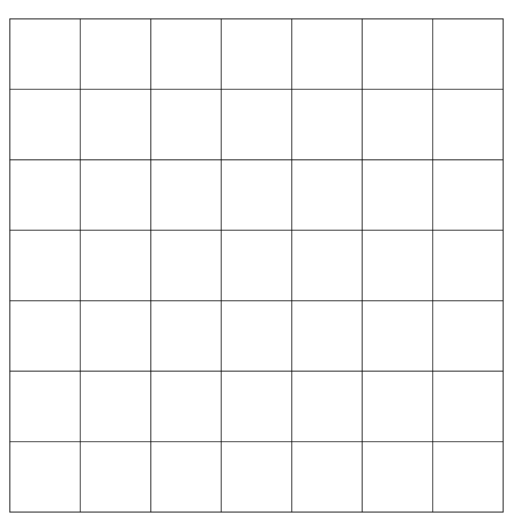
\includegraphics[scale=.3]{7x7.png}
\end{figure}
Our feature function for faces splits the datum into 42 parts and counts the number of black pixels in each part. The regions of the data look like below.\\
\begin{figure}[H]
  	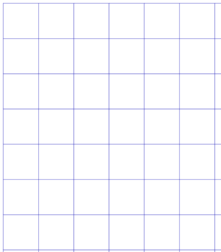
\includegraphics[scale=.6]{6x7.png}
\end{figure}
To count the number of black pixels in each part, we traverse through each pixel of a part and update the number of black pixels in that part. \\
We implemented several other feature functions in featureFuncLib.py but used the two above because they helped to give the best accuracy.

%----------------------------------------------------------------------------------------
%	SECTION 5
%----------------------------------------------------------------------------------------

\section{Naive Bayes Algorithm}

\subsection{Overview for Face Detection}

We want to calculate $L(x) =\dfrac{ p(y = true\mid x)}{p(y = f alse\mid x)} = \dfrac{p(x\mid y = true)p(y = true)}{p(x\mid y = f alse)p(y = f alse)}$. We return true if$ L(x) \geq1$ and false otherwise. \\\\
Our train function prepares all of the values necessary for calculating $p(x\mid y = true)$, $p(y = true)$, $p(x\mid y = f alse)$, $p(y = f alse)$ based on information in the train set.\\\\
Our predict function calculates L(x) for each item in the test set. Based on the L(x) value of an item, the predict function assigns a label of 0 or 1 to that item. A 0 represents that the item is not a face and 1 represents that the item is a face.
\subsection{Data Structures for Face Detection}
We have one probability array containing information necessary to calculate $p(x\mid y = true)$ and one probability array containing information necessary to calculate $p(x\mid y = false)$.\\\\
Each probability array is an array of dictionaries.\\\\
We use dictionaries because searching is O(1) time while searching in an array takes O(trainingsize) time.\\\\
The probability array has the following form:\\\\
\{dictionary containing (value, probability) pairs for feature 1\},\\\\
\{dictionary containing (value, probability) pairs for feature 2\},\\\\
\{dictionary containing (value, probability) pairs for feature 3\},…

\subsection{Method Definitions for Face Detection}
\textit{Train}\\\\
Input: train features, train labels\\\\
Output: P(face=true), P(face=not true), array1 as described below, array2 as described below\\\\
Where array1 is an array containing probabilities given that the image is a face. We organized the array to be an array of dictionaries; each dictionary represents a feature and contains (value, probability) pairs for the likelihood that the feature has that value, given that the image is a face. \\\\
Where array2 is an array containing probabilities given that the image is NOT a face. We organized the array to be an array of dictionaries; each dictionary represents a feature and contains (value, probability) pairs for the likelihood that the feature has that value, given that the image is not a face.\\\\
\textit{Predict} \\\\
Input: test features, pFace, pNotFace, array1, array2\\
Output: predicted labels\\

\subsection{Train Algorithm for Face Detection}

\begin{tabbing}
\textit{Part 0: This part initializes variables}\\
numberOfFaces=0\\
numberOfNotFaces=0\\
Array1=[ {} ,  {}, {}…]\\
Array2=[ {} ,  {}, {}…]\\\\
\textit{Part 1: This part finds counts}\\
For \=each feature array in the training set\\
	\>  If the \= label \=shows that the image IS A FACE\\
	\> \> 	numberOfFaces++\\
	\> \> 	for feature i in the array of features\\
	\> \> 	\> 	in array1, add feature i to the dictionary that corresponds to feature i and \\
	\> \> 	\> 	update the count that corresponds to feature i\\
	\>If the label shows the image IS NOT A FACE\\
	\> \>	numberOfNotFaces++\\
	\> \>	for feature i in the array of features\\
	\> \>\>	in array2, add feature i to the dictionary that corresponds to feature i and \\
	\> \> 	\> 	update the count that corresponds to feature i\\\\
\textit{Part 2: This part turns counts into probabilities}\\
For every count in array1, turn it into count/numberOfFaces\\
For every count in array2, turn it into count/numberOfNotFaces\\
pFace=numberOfFaces/total\\
pNotFace=numberOfNotFaces/total\\
return pFace, pNotFace, array1, array2\\ 
\end{tabbing}
\subsection{Predict Algorithm for Face Detection}

Need to calculate $p(x\mid y = true)$, $p(y = true)$, $p(x\mid y = f alse)$, $p(y = f alse)$

\begin{tabbing}
For \=each item in test features\\
	\> Use the formulas below to compute $p(x\mid y = true)$ from array1 and $p(x\mid y = f alse)$ from array2\\
	\> Then compute L(x)\\
	\> Then add label based on the L(x) value into the predict array
\end{tabbing}

\begin{figure}[H]
  	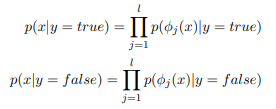
\includegraphics[scale=.7]{Formulas.png}
\end{figure}


\subsection{Overview for Digit Identification}

Instead of calculating L(x) as for face, calculate $p(x\mid y = true)*p(y = true)$ for each digit and predict the digit with the maximum result in this calculation. \\\\
The train and predict algorithm are very similar to that for face detection.
\subsection{Method Definitions for Digit Identification}
\textit{Train}\\\\
Input: train features, train labels\\
Output: P(digit 0=true), P(digit 1=true), P(digit 2=true), P(digit 3=true), P(digit 4=true), P(digit 5=true), P(digit 6=true), P(digit 7=true), P(digit 8=true), P(digit 9=true),  array0, array1, array2, array3, array4, array5, array6, array7, array8, array9\\\\
\textit{Predict}\\\\
Input: test features, test labels, P(digit 0=true), P(digit 1=true), P(digit 2=true), P(digit 3=true), P(digit 4=true), P(digit 5=true), P(digit 6=true), P(digit 7=true), P(digit 8=true), P(digit 9=true),  array0, array1, array2, array3, array4, array5, array6, array7, array8, array9\\
Output: predict\\

Where array1,2,...10 is an array containing probabilities given that the image is a face. We organized the array to be an array of dictionaries; each dictionary represents a feature and contains (value, probability) pairs for the likelihood that the feature has that value, given that the image is a face. \\\\


%----------------------------------------------------------------------------------------
%	SECTION 5
%----------------------------------------------------------------------------------------

\section{Perceptron}

\subsection{Overview for Face Detection}

We calculate $f(x_i , w) = w_0 + w_1\Phi_1(x_i) + w_2 \Phi_2(x_i) + w_3 \Phi_3(x_i) + ...+ w_l\Phi_l(x_i)$. If $f(x_i , w) \geq 0$, we predict that it is a face; otherwise, we predict that it is not a face. \\\\
Our train function prepares all of the weights necessary for calculating $f(x_i , w) = w_0 + w_1\Phi_1(x_i) + w_2 \Phi_2(x_i) + w_3 \Phi_3(x_i) + ...+ w_l\Phi_l(x_i)$ based on information in the train set.\\\\
Our predict function calculates $f(x_i,w)$ for each item in test set assigns a label of 0 or 1 to that item; a 0 represents that the item is not a face and 1 represents that the item is a face.
\subsection{Method Definition and Algorithm of Train for Face Detection}
Input: train features, train labels\\
Output: array of weights\\

Initialize weights as [0.0001]\\
Iterate through the train features and labels until you don’t have to adjust the weights anymore, or until a specific time has passed\\
Return weights\\

We specified the time limit to be 136 iterations. After the train function has completed 136 iterations of adjusting weights, it will return the array of weights as it exists after the 136 iterations.



\subsection{Method Definition and Algorithm of Predict for Face Detection}
Input: test features, array of weights\\
Output: predict labels\\

For each test feature array, calculate f(x)\\
Based on f(x), append 0 or 1 to the predict array, where 0 represents that the item is not a face and 1 represents that the item is a face.

\subsection{Overview for Digit Identification}

Instead of calculating one $f(x_i,w)$ function as in face indentification, calculate 10 of the them and choose the digit that corresponds to the maximum f value as the digit that the algorithm predicts for an image

\subsection{Method Definitions for Digit Identification}
\textit{Train}\\
Input: train features, train labels\\
Output: array of weights for digit 0, array of weights for digit 1, array of weights for digit 2, array of weights for digit 3, array of weights for digit 4, array of weights for digit 5, array of weights for digit 6, array of weights for digit 7, array of weights for digit 8, array of weights for digit 9\\\\
\textit{Predict}\\
Input: test features, array of weights for digit 0, array of weights for digit 1, array of weights for digit 2, array of weights for digit 3, array of weights for digit 4, array of weights for digit 5, array of weights for digit 6, array of weights for digit 7, array of weights for digit 8, array of weights for digit 9\\
Output: predict labels\\

We specified the time limit to be 175 iterations. After the train function has completed 175 iterations of adjusting weights, it will return the array of weights as it exists after the 175 iterations.

%----------------------------------------------------------------------------------------
%	SECTION 5
%----------------------------------------------------------------------------------------

\section{kNN}

Unlike the Naïve Bayes and Perceptron algorithms, kNN only has a predict function. The kNN algorithm takes in training features, training labels, test features, test labels, and a k value and returns an array of predicted labels for the test features. \\\\
For each array of features in the test set, the kNN algorithm looks through all of the arrays of features in the training set and chooses the k images that are most similar to the image in the test set. Then it uses the most frequent label of the k images to predict whether the current image in the test set is a face or not. \\\\
In our trials, we noticed that the prediction accuracy is highest when k=1. As a result, we recorded data from trials only when we assigned k to be 1.\\\\
However, our code works for any k-value. 

%----------------------------------------------------------------------------------------
%	SECTION 5
%----------------------------------------------------------------------------------------

\section{How We Compared the Algorithms}
In total, we wanted to compare the performace for 6 algorithms: Naive Bayes for face detection and digit identification, Perceptron for face detection and digit identification, and kNN for face detection and digit identification. We also wanted to compare the performance of these algorithms when using 10\%, 20\%... 100\% of the training set. \\

We ran each algorithm five times on each training set size. When the training set size was 40\% of the entire training data, we implemented an algorithm to randomly select 40\% of the entire training data during each of the five trials. As a result of the randomness, our algorithm has slightly different results in accuracy and training time.\\

Therefore, for each algorithm and training set size, we performed five trials. For each trial, we recorded the accuracy and the time necessary to train the algorithm. kNN does not have a training function; we could not calculate the time necessary to train the algorithm so we recorded the amount of time that the algorithm spent to predict one label for one image. \\

For each algorithm and training set size, we recorded the average accuracy, the standard deviation of the accuracy, and the average time needed to train the algorithm over all five trials. 


%----------------------------------------------------------------------------------------
%	SECTION 5
%----------------------------------------------------------------------------------------

\section{Analysis of the Naive Bayes Face Detection Algorithm on Each Training Set Size}

Our results for the Naive Bayes Face Detection Algorithm are below.

\begin{table}[H]

\centering
{\begin{tabular}{||p{1cm}|p{1.8cm}|p{1.8cm}|p{3cm}||}
 \hline
Trial & Accuracy & Error & Training time (seconds) \\ [0.5ex] 
 \hline\hline
   0  & 0.76  & 0.24  & 0.001\\
\hline
   1  & 0.73  & 0.27  & 0.002\\
\hline
   2  & 0.7  & 0.3  & 0.001\\
\hline
   3  & 0.64  & 0.36  & 0.001\\
\hline
   4  & 0.79  & 0.21  & 0.001\\
 \hline
\end{tabular}}
\caption{TRAINING SIZE: 10\% \newline Summary for Table 1 on a Training Size of 10\%: Mean Accuracy=0.72, Standard Deviation=0.05, Mean Error=0.28, Average Training Time (Seconds)=0.001}
\end{table} 

\begin{table}[H]

\centering
{\begin{tabular}{||p{1cm}|p{1.8cm}|p{1.8cm}|p{3cm}||}
 \hline
Trial & Accuracy & Error & Training time (seconds) \\ [0.5ex] 
 \hline\hline
   0  & 0.8  & 0.2  & 0.002\\
\hline
   1  & 0.7  & 0.3  & 0.002\\
\hline
   2  & 0.7  & 0.3  & 0.004\\
\hline
   3  & 0.74  & 0.26  & 0.002\\
\hline
   4  & 0.72  & 0.28  & 0.002\\
 \hline
\end{tabular}}
\caption{TRAINING SIZE: 20\% \newline Summary for Table 2 on a Training Size of 20\%: Mean Accuracy=0.73, Standard Deviation=0.04, Mean Error=0.27, Average Training Time (Seconds)=0.002}
\end{table} 

\begin{table}[H]

\centering
{\begin{tabular}{||p{1cm}|p{1.8cm}|p{1.8cm}|p{3cm}||}
 \hline
Trial & Accuracy & Error & Training time (seconds) \\ [0.5ex] 
 \hline\hline
   0  & 0.76  & 0.24  & 0.003\\
\hline
   1  & 0.8  & 0.2  & 0.003\\
\hline
   2  & 0.77  & 0.23  & 0.003\\
\hline
   3  & 0.82  & 0.18  & 0.003\\
\hline
   4  & 0.76  & 0.24  & 0.003\\
 \hline
\end{tabular}}
\caption{TRAINING SIZE: 30\% \newline Summary for Table 3 on a Training Size of 30\%: Mean Accuracy=0.78, Standard Deviation=0.02, Mean Error=0.22, Average Training Time (Seconds)=0.003}
\end{table} 

\begin{table}[H]

\centering
{\begin{tabular}{||p{1cm}|p{1.8cm}|p{1.8cm}|p{3cm}||}
 \hline
Trial & Accuracy & Error & Training time (seconds) \\ [0.5ex] 
 \hline\hline
   0  & 0.81  & 0.19  & 0.004\\
\hline
   1  & 0.84  & 0.16  & 0.004\\
\hline
   2  & 0.71  & 0.29  & 0.005\\
\hline
   3  & 0.69  & 0.31  & 0.004\\
\hline
   4  & 0.76  & 0.24  & 0.004\\
 \hline
\end{tabular}}
\caption{TRAINING SIZE: 40\% \newline Summary for Table 4 on a Training Size of 40\%: Mean Accuracy=0.76, Standard Deviation=0.06, Mean Error=0.24, Average Training Time (Seconds)=0.004}
\end{table} 

\begin{table}[H]

\centering
{\begin{tabular}{||p{1cm}|p{1.8cm}|p{1.8cm}|p{3cm}||}
 \hline
Trial & Accuracy & Error & Training time (seconds) \\ [0.5ex] 
 \hline\hline
0  & 0.78  & 0.22  & 0.005\\
\hline
   1  & 0.86  & 0.14  & 0.005\\
\hline
   2  & 0.8  & 0.2  & 0.005\\
\hline
   3  & 0.82  & 0.18  & 0.005\\
\hline
   4  & 0.78  & 0.22  & 0.005\\
 \hline
\end{tabular}}
\caption{TRAINING SIZE: 50\% \newline Summary for Table 5 on a Training Size of 50\%: Mean Accuracy=0.81, Standard Deviation=0.03, Mean Error=0.19, Average Training Time (Seconds)=0.005}
\end{table} 

\begin{table}[H]

\centering
{\begin{tabular}{||p{1cm}|p{1.8cm}|p{1.8cm}|p{3cm}||}
 \hline
Trial & Accuracy & Error & Training time (seconds) \\ [0.5ex] 
 \hline\hline
   0  & 0.76  & 0.24  & 0.007\\
\hline
   1  & 0.85  & 0.15  & 0.006\\
\hline
   2  & 0.8  & 0.2  & 0.007\\
\hline
   3  & 0.79  & 0.21  & 0.006\\
\hline
   4  & 0.78  & 0.22  & 0.006\\
 \hline
\end{tabular}}
\caption{TRAINING SIZE: 60\% \newline Summary for Table 6 on a Training Size of 60\%: Mean Accuracy=0.8, Standard Deviation=0.03, Mean Error=0.2, Average Training Time (Seconds)=0.006}
\end{table} 

\begin{table}[H]

\centering
{\begin{tabular}{||p{1cm}|p{1.8cm}|p{1.8cm}|p{3cm}||}
 \hline
Trial & Accuracy & Error & Training time (seconds) \\ [0.5ex] 
 \hline\hline
   0  & 0.84  & 0.16  & 0.007\\
\hline
   1  & 0.8  & 0.2  & 0.007\\
\hline
   2  & 0.79  & 0.21  & 0.008\\
\hline
   3  & 0.83  & 0.17  & 0.007\\
\hline
   4  & 0.78  & 0.22  & 0.007\\
 \hline
\end{tabular}}
\caption{TRAINING SIZE: 70\% \newline Summary for Table 7 on a Training Size of 70\%: Mean Accuracy=0.81, Standard Deviation=0.02, Mean Error=0.19, Average Training Time (Seconds)=0.007}
\end{table} 

\begin{table}[H]

\centering
{\begin{tabular}{||p{1cm}|p{1.8cm}|p{1.8cm}|p{3cm}||}
 \hline
Trial & Accuracy & Error & Training time (seconds) \\ [0.5ex] 
 \hline\hline
   0  & 0.84  & 0.16  & 0.008\\
\hline
   1  & 0.81  & 0.19  & 0.008\\
\hline
   2  & 0.86  & 0.14  & 0.009\\
\hline
   3  & 0.84  & 0.16  & 0.009\\
\hline
   4  & 0.84  & 0.16  & 0.008\\
 \hline
\end{tabular}}
\caption{TRAINING SIZE: 80\% \newline Summary for Table 8 on a Training Size of 80\%: Mean Accuracy=0.84, Standard Deviation=0.02, Mean Error=0.16, Average Training Time (Seconds)=0.008}
\end{table} 

\begin{table}[H]

\centering
{\begin{tabular}{||p{1cm}|p{1.8cm}|p{1.8cm}|p{3cm}||}
 \hline
Trial & Accuracy & Error & Training time (seconds) \\ [0.5ex] 
 \hline\hline
   0  & 0.88  & 0.12  & 0.009\\
\hline
   1  & 0.84  & 0.16  & 0.009\\
\hline
   2  & 0.85  & 0.15  & 0.009\\
\hline
   3  & 0.86  & 0.14  & 0.009\\
\hline
   4  & 0.88  & 0.12  & 0.01\\
 \hline
\end{tabular}}
\caption{TRAINING SIZE: 90\% \newline Summary for Table 9 on a Training Size of 90\%: Mean Accuracy=0.86, Standard Deviation=0.02, Mean Error=0.14, Average Training Time (Seconds)=0.009}
\end{table} 

\begin{table}[H]

\centering
{\begin{tabular}{||p{1cm}|p{1.8cm}|p{1.8cm}|p{3cm}||}
 \hline
Trial & Accuracy & Error & Training time (seconds) \\ [0.5ex] 
 \hline\hline
   0  & 0.88  & 0.12  & 0.011\\
\hline
   1  & 0.88  & 0.12  & 0.01\\
\hline
   2  & 0.88  & 0.12  & 0.011\\
\hline
   3  & 0.88  & 0.12  & 0.01\\
\hline
   4  & 0.88  & 0.12  & 0.011\\
 \hline
\end{tabular}}
\caption{TRAINING SIZE: 100\% \newline Summary for Table 10 on a Training Size of 100\%: Mean Accuracy=0.88, Standard Deviation=0.0, Mean Error=0.12, Average Training Time (Seconds)=0.011}
\end{table} 

%----------------------------------------------------------------------------------------
%	SECTION 5
%----------------------------------------------------------------------------------------

\section{Analysis of the Naive Bayes Digit Identification Algorithm on Each Training Set Size}

Our results for the Naive Bayes Digit Identification Algorithm are below.

\begin{table}[H]

\centering
{\begin{tabular}{||p{1cm}|p{1.8cm}|p{1.8cm}|p{3cm}||}
 \hline
Trial & Accuracy & Error & Training time (seconds) \\ [0.5ex] 
 \hline\hline
   0  & 0.64  & 0.36  & 0.014\\
\hline
   1  & 0.69  & 0.31  & 0.014\\
\hline
   2  & 0.68  & 0.32  & 0.013\\
\hline
   3  & 0.58  & 0.42  & 0.013\\
\hline
   4  & 0.59  & 0.41  & 0.014\\
\hline

\end{tabular}}
\caption{TRAINING SIZE: 10\% \newline Summary for Table 11 on a Training Size of 10\%: Mean Accuracy=0.64, Standard Deviation=0.04, Mean Error=0.36, Average Training Time (Seconds)=0.014}
\end{table} 

\begin{table}[H]

\centering
{\begin{tabular}{||p{1cm}|p{1.8cm}|p{1.8cm}|p{3cm}||}
 \hline
Trial & Accuracy & Error & Training time (seconds) \\ [0.5ex] 
 \hline\hline
   0  & 0.69  & 0.31  & 0.028\\
\hline
   1  & 0.69  & 0.31  & 0.028\\
\hline
   2  & 0.69  & 0.31  & 0.028\\
\hline
   3  & 0.68  & 0.32  & 0.028\\
\hline
   4  & 0.72  & 0.28  & 0.028\\
\hline

\end{tabular}}
\caption{TRAINING SIZE: 20\% \newline Summary for Table 12 on a Training Size of 20\%: Mean Accuracy=0.69, Standard Deviation=0.01, Mean Error=0.31, Average Training Time (Seconds)=0.028}
\end{table} 

\begin{table}[H]

\centering
{\begin{tabular}{||p{1cm}|p{1.8cm}|p{1.8cm}|p{3cm}||}
 \hline
Trial & Accuracy & Error & Training time (seconds) \\ [0.5ex] 
 \hline\hline
   0  & 0.7  & 0.3  & 0.041\\
\hline
   1  & 0.83  & 0.17  & 0.042\\
\hline
   2  & 0.76  & 0.24  & 0.041\\
\hline
   3  & 0.74  & 0.26  & 0.042\\
\hline
   4  & 0.75  & 0.25  & 0.042\\
\hline

\end{tabular}}
\caption{TRAINING SIZE: 30\% \newline Summary for Table 13 on a Training Size of 30\%: Mean Accuracy=0.76, Standard Deviation=0.04, Mean Error=0.24, Average Training Time (Seconds)=0.042}
\end{table} 

\begin{table}[H]

\centering
{\begin{tabular}{||p{1cm}|p{1.8cm}|p{1.8cm}|p{3cm}||}
 \hline
Trial & Accuracy & Error & Training time (seconds) \\ [0.5ex] 
 \hline\hline
   0  & 0.75  & 0.25  & 0.055\\
\hline
   1  & 0.76  & 0.24  & 0.055\\
\hline
   2  & 0.76  & 0.24  & 0.055\\
\hline
   3  & 0.76  & 0.24  & 0.055\\
\hline
   4  & 0.74  & 0.26  & 0.057\\
\hline

\end{tabular}}
\caption{TRAINING SIZE: 40\% \newline Summary for Table 14 on a Training Size of 40\%: Mean Accuracy=0.75, Standard Deviation=0.01, Mean Error=0.25, Average Training Time (Seconds)=0.055}
\end{table} 

\begin{table}[H]

\centering
{\begin{tabular}{||p{1cm}|p{1.8cm}|p{1.8cm}|p{3cm}||}
 \hline
Trial & Accuracy & Error & Training time (seconds) \\ [0.5ex] 
 \hline\hline
   0  & 0.76  & 0.24  & 0.069\\
\hline
   1  & 0.78  & 0.22  & 0.069\\
\hline
   2  & 0.8  & 0.2  & 0.069\\
\hline
   3  & 0.77  & 0.23  & 0.069\\
\hline
   4  & 0.78  & 0.22  & 0.07\\
\hline

\end{tabular}}
\caption{TRAINING SIZE: 50\% \newline Summary for Table 15 on a Training Size of 50\%: Mean Accuracy=0.78, Standard Deviation=0.01, Mean Error=0.22, Average Training Time (Seconds)=0.069}
\end{table} 

\begin{table}[H]

\centering
{\begin{tabular}{||p{1cm}|p{1.8cm}|p{1.8cm}|p{3cm}||}
 \hline
Trial & Accuracy & Error & Training time (seconds) \\ [0.5ex] 
 \hline\hline
   0  & 0.8  & 0.2  & 0.083\\
\hline
   1  & 0.79  & 0.21  & 0.089\\
\hline
   2  & 0.81  & 0.19  & 0.084\\
\hline
   3  & 0.79  & 0.21  & 0.085\\
\hline
   4  & 0.8  & 0.2  & 0.085\\
\hline

\end{tabular}}
\caption{TRAINING SIZE: 60\% \newline Summary for Table 16 on a Training Size of 60\%: Mean Accuracy=0.8, Standard Deviation=0.01, Mean Error=0.2, Average Training Time (Seconds)=0.085}
\end{table} 

\begin{table}[H]

\centering
{\begin{tabular}{||p{1cm}|p{1.8cm}|p{1.8cm}|p{3cm}||}
 \hline
Trial & Accuracy & Error & Training time (seconds) \\ [0.5ex] 
 \hline\hline
   0  & 0.77  & 0.23  & 0.097\\
\hline
   1  & 0.82  & 0.18  & 0.097\\
\hline
   2  & 0.81  & 0.19  & 0.096\\
\hline
   3  & 0.82  & 0.18  & 0.098\\
\hline
   4  & 0.82  & 0.18  & 0.098\\
\hline

\end{tabular}}
\caption{TRAINING SIZE: 70\% \newline Summary for Table 17 on a Training Size of 70\%: Mean Accuracy=0.81, Standard Deviation=0.02, Mean Error=0.19, Average Training Time (Seconds)=0.097}
\end{table} 

\begin{table}[H]

\centering
{\begin{tabular}{||p{1cm}|p{1.8cm}|p{1.8cm}|p{3cm}||}
 \hline
Trial & Accuracy & Error & Training time (seconds) \\ [0.5ex] 
 \hline\hline
   0  & 0.78  & 0.22  & 0.115\\
\hline
   1  & 0.77  & 0.23  & 0.112\\
\hline
   2  & 0.8  & 0.2  & 0.116\\
\hline
   3  & 0.81  & 0.19  & 0.113\\
\hline
   4  & 0.79  & 0.21  & 0.112\\
\hline

\end{tabular}}
\caption{TRAINING SIZE: 80\% \newline Summary for Table 18 on a Training Size of 80\%: Mean Accuracy=0.79, Standard Deviation=0.01, Mean Error=0.21, Average Training Time (Seconds)=0.114}
\end{table} 

\begin{table}[H]

\centering
{\begin{tabular}{||p{1cm}|p{1.8cm}|p{1.8cm}|p{3cm}||}
 \hline
Trial & Accuracy & Error & Training time (seconds) \\ [0.5ex] 
 \hline\hline
   0  & 0.82  & 0.18  & 0.126\\
\hline
   1  & 0.82  & 0.18  & 0.127\\
\hline
   2  & 0.8  & 0.2  & 0.126\\
\hline
   3  & 0.79  & 0.21  & 0.127\\
\hline
   4  & 0.8  & 0.2  & 0.126\\
\hline

\end{tabular}}
\caption{TRAINING SIZE: 90\% \newline Summary for Table 19 on a Training Size of 90\%: Mean Accuracy=0.81, Standard Deviation=0.01, Mean Error=0.19, Average Training Time (Seconds)=0.126}
\end{table} 

\begin{table}[H]

\centering
{\begin{tabular}{||p{1cm}|p{1.8cm}|p{1.8cm}|p{3cm}||}
 \hline
Trial & Accuracy & Error & Training time (seconds) \\ [0.5ex] 
 \hline\hline
   0  & 0.81  & 0.19  & 0.145\\
\hline
   1  & 0.81  & 0.19  & 0.141\\
\hline
   2  & 0.81  & 0.19  & 0.141\\
\hline
   3  & 0.81  & 0.19  & 0.142\\
\hline
   4  & 0.81  & 0.19  & 0.139\\
\hline

\end{tabular}}
\caption{TRAINING SIZE: 100\% \newline Summary for Table 20 on a Training Size of 100\%: Mean Accuracy=0.81, Standard Deviation=0.0, Mean Error=0.19, Average Training Time (Seconds)=0.142}
\end{table} 

%----------------------------------------------------------------------------------------
%	SECTION 5
%----------------------------------------------------------------------------------------

\section{Analysis of the Perceptron Face Detection Algorithm on Each Training Set Size}

Our results for the Perceptron Face Detection Algorithm are below.

\begin{table}[H]

\centering
{\begin{tabular}{||p{1cm}|p{1.8cm}|p{1.8cm}|p{3cm}||}
 \hline
Trial & Accuracy & Error & Training time (seconds) \\ [0.5ex] 
 \hline\hline
   0 & 0.68 & 0.32 & 0.004\\
\hline
   1 & 0.8 & 0.2 & 0.011\\
\hline
   2 & 0.7 & 0.3 & 0.013\\
\hline
   3 & 0.72 & 0.28 & 0.007\\
\hline
   4 & 0.67 & 0.33 & 0.02\\
\hline
\end{tabular}}
\caption{TRAINING SIZE: 10\% \newline Summary for Table 21 on a Training Size of 10\%: Mean Accuracy=0.71, Standard Deviation=0.05, Mean Error=0.29, Average Training Time (Seconds)=0.011}
\end{table} 

\begin{table}[H]

\centering
{\begin{tabular}{||p{1cm}|p{1.8cm}|p{1.8cm}|p{3cm}||}
 \hline
Trial & Accuracy & Error & Training time (seconds) \\ [0.5ex] 
 \hline\hline
   0 & 0.69 & 0.31 & 0.113\\
\hline
   1 & 0.68 & 0.32 & 0.084\\
\hline
   2 & 0.63 & 0.37 & 0.113\\
\hline
   3 & 0.8 & 0.2 & 0.109\\
\hline
   4 & 0.73 & 0.27 & 0.052\\
\hline
\end{tabular}}
\caption{TRAINING SIZE: 20\% \newline Summary for Table 22 on a Training Size of 20\%: Mean Accuracy=0.71, Standard Deviation=0.06, Mean Error=0.29, Average Training Time (Seconds)=0.094}
\end{table} 

\begin{table}[H]

\centering
{\begin{tabular}{||p{1cm}|p{1.8cm}|p{1.8cm}|p{3cm}||}
 \hline
Trial & Accuracy & Error & Training time (seconds) \\ [0.5ex] 
 \hline\hline
   0 & 0.67 & 0.33 & 0.181\\
\hline
   1 & 0.76 & 0.24 & 0.178\\
\hline
   2 & 0.71 & 0.29 & 0.169\\
\hline
   3 & 0.75 & 0.25 & 0.178\\
\hline
   4 & 0.68 & 0.32 & 0.181\\
\hline
\end{tabular}}
\caption{TRAINING SIZE: 30\% \newline Summary for Table 23 on a Training Size of 30\%: Mean Accuracy=0.71, Standard Deviation=0.04, Mean Error=0.29, Average Training Time (Seconds)=0.177}
\end{table} 

\begin{table}[H]

\centering
{\begin{tabular}{||p{1cm}|p{1.8cm}|p{1.8cm}|p{3cm}||}
 \hline
Trial & Accuracy & Error & Training time (seconds) \\ [0.5ex] 
 \hline\hline
   0 & 0.79 & 0.21 & 0.218\\
\hline
   1 & 0.73 & 0.27 & 0.226\\
\hline
   2 & 0.72 & 0.28 & 0.238\\
\hline
   3 & 0.8 & 0.2 & 0.242\\
\hline
   4 & 0.77 & 0.23 & 0.24\\
\hline
\end{tabular}}
\caption{TRAINING SIZE: 40\% \newline Summary for Table 24 on a Training Size of 40\%: Mean Accuracy=0.76, Standard Deviation=0.03, Mean Error=0.24, Average Training Time (Seconds)=0.233}
\end{table} 

\begin{table}[H]

\centering
{\begin{tabular}{||p{1cm}|p{1.8cm}|p{1.8cm}|p{3cm}||}
 \hline
Trial & Accuracy & Error & Training time (seconds) \\ [0.5ex] 
 \hline\hline
   0 & 0.65 & 0.35 & 0.322\\
\hline
   1 & 0.75 & 0.25 & 0.298\\
\hline
   2 & 0.75 & 0.25 & 0.301\\
\hline
   3 & 0.76 & 0.24 & 0.296\\
\hline
   4 & 0.72 & 0.28 & 0.31\\
\hline
\end{tabular}}
\caption{TRAINING SIZE: 50\% \newline Summary for Table 25 on a Training Size of 50\%: Mean Accuracy=0.73, Standard Deviation=0.04, Mean Error=0.27, Average Training Time (Seconds)=0.305}
\end{table} 

\begin{table}[H]

\centering
{\begin{tabular}{||p{1cm}|p{1.8cm}|p{1.8cm}|p{3cm}||}
 \hline
Trial & Accuracy & Error & Training time (seconds) \\ [0.5ex] 
 \hline\hline
   0 & 0.74 & 0.26 & 0.363\\
\hline
   1 & 0.77 & 0.23 & 0.366\\
\hline
   2 & 0.71 & 0.29 & 0.358\\
\hline
   3 & 0.73 & 0.27 & 0.364\\
\hline
   4 & 0.75 & 0.25 & 0.361\\
\hline
\end{tabular}}
\caption{TRAINING SIZE: 60\% \newline Summary for Table 26 on a Training Size of 60\%: Mean Accuracy=0.74, Standard Deviation=0.02, Mean Error=0.26, Average Training Time (Seconds)=0.362}
\end{table} 

\begin{table}[H]

\centering
{\begin{tabular}{||p{1cm}|p{1.8cm}|p{1.8cm}|p{3cm}||}
 \hline
Trial & Accuracy & Error & Training time (seconds) \\ [0.5ex] 
 \hline\hline
   0 & 0.75 & 0.25 & 0.437\\
\hline
   1 & 0.77 & 0.23 & 0.448\\
\hline
   2 & 0.77 & 0.23 & 0.427\\
\hline
   3 & 0.8 & 0.2 & 0.429\\
\hline
   4 & 0.74 & 0.26 & 0.433\\
\hline
\end{tabular}}
\caption{TRAINING SIZE: 70\% \newline Summary for Table 27 on a Training Size of 70\%: Mean Accuracy=0.77, Standard Deviation=0.02, Mean Error=0.23, Average Training Time (Seconds)=0.435}
\end{table} 

\begin{table}[H]

\centering
{\begin{tabular}{||p{1cm}|p{1.8cm}|p{1.8cm}|p{3cm}||}
 \hline
Trial & Accuracy & Error & Training time (seconds) \\ [0.5ex] 
 \hline\hline
   0 & 0.77 & 0.23 & 0.496\\
\hline
   1 & 0.74 & 0.26 & 0.493\\
\hline
   2 & 0.7 & 0.3 & 0.499\\
\hline
   3 & 0.72 & 0.28 & 0.496\\
\hline
   4 & 0.71 & 0.29 & 0.49\\
\hline
\end{tabular}}
\caption{TRAINING SIZE: 80\% \newline Summary for Table 28 on a Training Size of 80\%: Mean Accuracy=0.73, Standard Deviation=0.02, Mean Error=0.27, Average Training Time (Seconds)=0.495}
\end{table} 

\begin{table}[H]

\centering
{\begin{tabular}{||p{1cm}|p{1.8cm}|p{1.8cm}|p{3cm}||}
 \hline
Trial & Accuracy & Error & Training time (seconds) \\ [0.5ex] 
 \hline\hline
   0 & 0.76 & 0.24 & 0.562\\
\hline
   1 & 0.71 & 0.29 & 0.56\\
\hline
   2 & 0.75 & 0.25 & 0.552\\
\hline
   3 & 0.77 & 0.23 & 0.57\\
\hline
   4 & 0.78 & 0.22 & 0.558\\
\hline
\end{tabular}}
\caption{TRAINING SIZE: 90\% \newline Summary for Table 29 on a Training Size of 90\%: Mean Accuracy=0.75, Standard Deviation=0.02, Mean Error=0.25, Average Training Time (Seconds)=0.56}
\end{table} 

\begin{table}[H]

\centering
{\begin{tabular}{||p{1cm}|p{1.8cm}|p{1.8cm}|p{3cm}||}
 \hline
Trial & Accuracy & Error & Training time (seconds) \\ [0.5ex] 
 \hline\hline
   0 & 0.81 & 0.19 & 0.63\\
\hline
   1 & 0.78 & 0.22 & 0.628\\
\hline
   2 & 0.78 & 0.22 & 0.627\\
\hline
   3 & 0.76 & 0.24 & 0.629\\
\hline
   4 & 0.79 & 0.21 & 0.629\\
\hline
\end{tabular}}
\caption{TRAINING SIZE: 100\% \newline Summary for Table 30 on a Training Size of 100\%: Mean Accuracy=0.78, Standard Deviation=0.02, Mean Error=0.22, Average Training Time (Seconds)=0.629}
\end{table} 

%----------------------------------------------------------------------------------------
%	SECTION 5
%----------------------------------------------------------------------------------------

\section{Analysis of the Perceptron Digit Identification Algorithm on Each Training Set Size}

Our results for the Perceptron Digit Identification Algorithm are below.

\begin{table}[H]

\centering
{\begin{tabular}{||p{1cm}|p{1.8cm}|p{1.8cm}|p{3cm}||}
 \hline
Trial & Accuracy & Error & Training time (seconds) \\ [0.5ex] 
 \hline\hline
   0  & 0.71  & 0.29  & 8.239\\
\hline
   1  & 0.73  & 0.27  & 7.127\\
\hline
   2  & 0.77  & 0.23  & 8.173\\
\hline
   3  & 0.62  & 0.38  & 8.107\\
\hline
   4  & 0.64  & 0.36  & 7.247\\
\hline
\end{tabular}}
\caption{TRAINING SIZE: 10\% \newline Summary for Table 31 on a Training Size of 10\%: Mean Accuracy=0.69, Standard Deviation=0.06, Mean Error=0.31, Average Training Time (Seconds)=7.779}
\end{table} 

\begin{table}[H]

\centering
{\begin{tabular}{||p{1cm}|p{1.8cm}|p{1.8cm}|p{3cm}||}
 \hline
Trial & Accuracy & Error & Training time (seconds) \\ [0.5ex] 
 \hline\hline
   0  & 0.72  & 0.28  & 18.35\\
\hline
   1  & 0.74  & 0.26  & 17.803\\
\hline
   2  & 0.76  & 0.24  & 17.615\\
\hline
   3  & 0.76  & 0.24  & 17.5\\
\hline
   4  & 0.78  & 0.22  & 15.661\\
\hline
\end{tabular}}
\caption{TRAINING SIZE: 20\% \newline Summary for Table 32 on a Training Size of 20\%: Mean Accuracy=0.75, Standard Deviation=0.02, Mean Error=0.25, Average Training Time (Seconds)=17.386}
\end{table} 

\begin{table}[H]

\centering
{\begin{tabular}{||p{1cm}|p{1.8cm}|p{1.8cm}|p{3cm}||}
 \hline
Trial & Accuracy & Error & Training time (seconds) \\ [0.5ex] 
 \hline\hline
   0  & 0.79  & 0.21  & 26.515\\
\hline
   1  & 0.74  & 0.26  & 26.519\\
\hline
   2  & 0.71  & 0.29  & 26.719\\
\hline
   3  & 0.71  & 0.29  & 26.493\\
\hline
   4  & 0.78  & 0.22  & 26.458\\
\hline
\end{tabular}}
\caption{TRAINING SIZE: 30\% \newline Summary for Table 33 on a Training Size of 30\%: Mean Accuracy=0.75, Standard Deviation=0.03, Mean Error=0.25, Average Training Time (Seconds)=26.54}
\end{table} 

\begin{table}[H]

\centering
{\begin{tabular}{||p{1cm}|p{1.8cm}|p{1.8cm}|p{3cm}||}
 \hline
Trial & Accuracy & Error & Training time (seconds) \\ [0.5ex] 
 \hline\hline
   0  & 0.7  & 0.3  & 35.74\\
\hline
   1  & 0.65  & 0.35  & 35.296\\
\hline
   2  & 0.69  & 0.31  & 35.645\\
\hline
   3  & 0.75  & 0.25  & 35.338\\
\hline
   4  & 0.77  & 0.23  & 35.317\\
\hline
\end{tabular}}
\caption{TRAINING SIZE: 40\% \newline Summary for Table 34 on a Training Size of 40\%: Mean Accuracy=0.71, Standard Deviation=0.04, Mean Error=0.29, Average Training Time (Seconds)=35.467}
\end{table} 

\begin{table}[H]

\centering
{\begin{tabular}{||p{1cm}|p{1.8cm}|p{1.8cm}|p{3cm}||}
 \hline
Trial & Accuracy & Error & Training time (seconds) \\ [0.5ex] 
 \hline\hline
   0  & 0.73  & 0.27  & 44.312\\
\hline
   1  & 0.78  & 0.22  & 44.512\\
\hline
   2  & 0.77  & 0.23  & 44.602\\
\hline
   3  & 0.8  & 0.2  & 44.578\\
\hline
   4  & 0.82  & 0.18  & 44.261\\
\hline
\end{tabular}}
\caption{TRAINING SIZE: 50\% \newline Summary for Table 35 on a Training Size of 50\%: Mean Accuracy=0.78, Standard Deviation=0.03, Mean Error=0.22, Average Training Time (Seconds)=44.453}
\end{table} 

\begin{table}[H]

\centering
{\begin{tabular}{||p{1cm}|p{1.8cm}|p{1.8cm}|p{3cm}||}
 \hline
Trial & Accuracy & Error & Training time (seconds) \\ [0.5ex] 
 \hline\hline
   0  & 0.77  & 0.23  & 53.416\\
\hline
   1  & 0.76  & 0.24  & 53.193\\
\hline
   2  & 0.69  & 0.31  & 54.296\\
\hline
   3  & 0.86  & 0.14  & 53.523\\
\hline
   4  & 0.78  & 0.22  & 53.393\\
\hline
\end{tabular}}
\caption{TRAINING SIZE: 60\% \newline Summary for Table 36 on a Training Size of 60\%: Mean Accuracy=0.77, Standard Deviation=0.05, Mean Error=0.23, Average Training Time (Seconds)=53.564}
\end{table} 

\begin{table}[H]

\centering
{\begin{tabular}{||p{1cm}|p{1.8cm}|p{1.8cm}|p{3cm}||}
 \hline
Trial & Accuracy & Error & Training time (seconds) \\ [0.5ex] 
 \hline\hline
   0  & 0.8  & 0.2  & 62.602\\
\hline
   1  & 0.77  & 0.23  & 62.664\\
\hline
   2  & 0.81  & 0.19  & 62.719\\
\hline
   3  & 0.77  & 0.23  & 63.035\\
\hline
   4  & 0.81  & 0.19  & 63.752\\
\hline
\end{tabular}}
\caption{TRAINING SIZE: 70\% \newline Summary for Table 37 on a Training Size of 70\%: Mean Accuracy=0.79, Standard Deviation=0.02, Mean Error=0.21, Average Training Time (Seconds)=62.954}
\end{table} 

\begin{table}[H]

\centering
{\begin{tabular}{||p{1cm}|p{1.8cm}|p{1.8cm}|p{3cm}||}
 \hline
Trial & Accuracy & Error & Training time (seconds) \\ [0.5ex] 
 \hline\hline
   0  & 0.78  & 0.22  & 72.469\\
\hline
   1  & 0.78  & 0.22  & 72.138\\
\hline
   2  & 0.79  & 0.21  & 73.232\\
\hline
   3  & 0.73  & 0.27  & 72.964\\
\hline
   4  & 0.79  & 0.21  & 74.094\\
\hline
\end{tabular}}
\caption{TRAINING SIZE: 80\% \newline Summary for Table 38 on a Training Size of 80\%: Mean Accuracy=0.77, Standard Deviation=0.02, Mean Error=0.23, Average Training Time (Seconds)=72.98}
\end{table} 

\begin{table}[H]

\centering
{\begin{tabular}{||p{1cm}|p{1.8cm}|p{1.8cm}|p{3cm}||}
 \hline
Trial & Accuracy & Error & Training time (seconds) \\ [0.5ex] 
 \hline\hline
   0  & 0.77  & 0.23  & 84.443\\
\hline
   1  & 0.76  & 0.24  & 83.723\\
\hline
   2  & 0.78  & 0.22  & 84.17\\
\hline
   3  & 0.75  & 0.25  & 83.871\\
\hline
   4  & 0.78  & 0.22  & 84.22\\
\hline
\end{tabular}}
\caption{TRAINING SIZE: 90\% \newline Summary for Table 39 on a Training Size of 90\%: Mean Accuracy=0.77, Standard Deviation=0.01, Mean Error=0.23, Average Training Time (Seconds)=84.085}
\end{table} 

\begin{table}[H]

\centering
{\begin{tabular}{||p{1cm}|p{1.8cm}|p{1.8cm}|p{3cm}||}
 \hline
Trial & Accuracy & Error & Training time (seconds) \\ [0.5ex] 
 \hline\hline
   0  & 0.73  & 0.27  & 93.306\\
\hline
   1  & 0.78  & 0.22  & 91.718\\
\hline
   2  & 0.7  & 0.3  & 89.916\\
\hline
   3  & 0.72  & 0.28  & 89.939\\
\hline
   4  & 0.76  & 0.24  & 90.01\\
\hline
\end{tabular}}
\caption{TRAINING SIZE: 100\% \newline Summary for Table 40 on a Training Size of 100\%: Mean Accuracy=0.74, Standard Deviation=0.03, Mean Error=0.26, Average Training Time (Seconds)=90.978}
\end{table} 

%----------------------------------------------------------------------------------------
%	SECTION 5
%----------------------------------------------------------------------------------------

\section{Analysis of the kNN Face Detection Algorithm on Each Training Set Size}

Our results for the kNN Face Detection Algorithm are below.\\

\begin{table}[H]

\centering
{\begin{tabular}{||p{1cm}|p{1.8cm}|p{1.8cm}|p{3cm}||}
 \hline
Trial & Accuracy & Error & Prediction Time Per Image (seconds) \\ [0.5ex] 
 \hline\hline
    0  & 0.7  & 0.3  & 0.001\\
\hline
    1  & 0.65  & 0.35  & 0.001\\
\hline
    2  & 0.65  & 0.35  & 0.001\\
\hline
    3  & 0.69  & 0.31  & 0.001\\
\hline
    4  & 0.62  & 0.38  & 0.001\\
\hline
\end{tabular}}
\caption{TRAINING SIZE: 10\% \newline Summary for Table 41 on a Training Size of 10\%: Mean Accuracy=0.66, Standard Deviation=0.03, Mean Error=0.34, Average Prediction Time Per Image (Seconds)=0.001}
\end{table} 

\begin{table}[H]

\centering
{\begin{tabular}{||p{1cm}|p{1.8cm}|p{1.8cm}|p{3cm}||}
 \hline
Trial & Accuracy & Error & Prediction Time Per Image (seconds) \\ [0.5ex] 
 \hline\hline
    0  & 0.69  & 0.31  & 0.001\\
\hline
    1  & 0.71  & 0.29  & 0.001\\
\hline
    2  & 0.59  & 0.41  & 0.001\\
\hline
    3  & 0.61  & 0.39  & 0.002\\
\hline
    4  & 0.63  & 0.37  & 0.002\\
\hline

\end{tabular}}
\caption{TRAINING SIZE: 20\% \newline Summary for Table 42 on a Training Size of 20\%: Mean Accuracy=0.65, Standard Deviation=0.05, Mean Error=0.35, Average Prediction Time Per Image (Seconds)=0.001}
\end{table} 

\begin{table}[H]

\centering
{\begin{tabular}{||p{1cm}|p{1.8cm}|p{1.8cm}|p{3cm}||}
 \hline
Trial & Accuracy & Error & Prediction Time Per Image (seconds) \\ [0.5ex] 
 \hline\hline
    0  & 0.74  & 0.26  & 0.002\\
\hline
    1  & 0.68  & 0.32  & 0.002\\
\hline
    2  & 0.74  & 0.26  & 0.002\\
\hline
    3  & 0.74  & 0.26  & 0.002\\
\hline
    4  & 0.65  & 0.35  & 0.002\\
\hline

\end{tabular}}
\caption{TRAINING SIZE: 30\% \newline Summary for Table 43 on a Training Size of 30\%: Mean Accuracy=0.71, Standard Deviation=0.04, Mean Error=0.29, Average Prediction Time Per Image (Seconds)=0.002}
\end{table} 

\begin{table}[H]

\centering
{\begin{tabular}{||p{1cm}|p{1.8cm}|p{1.8cm}|p{3cm}||}
 \hline
Trial & Accuracy & Error & Prediction Time Per Image (seconds) \\ [0.5ex] 
 \hline\hline
    0  & 0.67  & 0.33  & 0.003\\
\hline
    1  & 0.66  & 0.34  & 0.003\\
\hline
    2  & 0.72  & 0.28  & 0.003\\
\hline
    3  & 0.68  & 0.32  & 0.003\\
\hline
    4  & 0.68  & 0.32  & 0.003\\
\hline

\end{tabular}}
\caption{TRAINING SIZE: 40\% \newline Summary for Table 44 on a Training Size of 40\%: Mean Accuracy=0.68, Standard Deviation=0.02, Mean Error=0.32, Average Prediction Time Per Image (Seconds)=0.003}
\end{table} 

\begin{table}[H]

\centering
{\begin{tabular}{||p{1cm}|p{1.8cm}|p{1.8cm}|p{3cm}||}
 \hline
Trial & Accuracy & Error & Prediction Time Per Image (seconds) \\ [0.5ex] 
 \hline\hline
    0  & 0.72  & 0.28  & 0.004\\
\hline
    1  & 0.69  & 0.31  & 0.004\\
\hline
    2  & 0.69  & 0.31  & 0.004\\
\hline
    3  & 0.69  & 0.31  & 0.004\\
\hline
    4  & 0.69  & 0.31  & 0.004\\
\hline

\end{tabular}}
\caption{TRAINING SIZE: 50\% \newline Summary for Table 45 on a Training Size of 50\%: Mean Accuracy=0.7, Standard Deviation=0.01, Mean Error=0.3, Average Prediction Time Per Image (Seconds)=0.004}
\end{table} 

\begin{table}[H]

\centering
{\begin{tabular}{||p{1cm}|p{1.8cm}|p{1.8cm}|p{3cm}||}
 \hline
Trial & Accuracy & Error & Prediction Time Per Image (seconds) \\ [0.5ex] 
 \hline\hline
    0  & 0.72  & 0.28  & 0.004\\
\hline
    1  & 0.72  & 0.28  & 0.004\\
\hline
    2  & 0.75  & 0.25  & 0.004\\
\hline
    3  & 0.72  & 0.28  & 0.004\\
\hline
    4  & 0.69  & 0.31  & 0.004\\
\hline

\end{tabular}}
\caption{TRAINING SIZE: 60\% \newline Summary for Table 46 on a Training Size of 60\%: Mean Accuracy=0.72, Standard Deviation=0.02, Mean Error=0.28, Average Prediction Time Per Image (Seconds)=0.004}
\end{table} 

\begin{table}[H]

\centering
{\begin{tabular}{||p{1cm}|p{1.8cm}|p{1.8cm}|p{3cm}||}
 \hline
Trial & Accuracy & Error & Prediction Time Per Image (seconds) \\ [0.5ex] 
 \hline\hline
    0  & 0.69  & 0.31  & 0.005\\
\hline
    1  & 0.67  & 0.33  & 0.005\\
\hline
    2  & 0.71  & 0.29  & 0.005\\
\hline
    3  & 0.65  & 0.35  & 0.005\\
\hline
    4  & 0.76  & 0.24  & 0.005\\
\hline

\end{tabular}}
\caption{TRAINING SIZE: 70\% \newline Summary for Table 47 on a Training Size of 70\%: Mean Accuracy=0.7, Standard Deviation=0.04, Mean Error=0.3, Average Prediction Time Per Image (Seconds)=0.005}
\end{table} 

\begin{table}[H]

\centering
{\begin{tabular}{||p{1cm}|p{1.8cm}|p{1.8cm}|p{3cm}||}
 \hline
Trial & Accuracy & Error & Prediction Time Per Image (seconds) \\ [0.5ex] 
 \hline\hline
    0  & 0.73  & 0.27  & 0.006\\
\hline
    1  & 0.7  & 0.3  & 0.006\\
\hline
    2  & 0.7  & 0.3  & 0.006\\
\hline
    3  & 0.74  & 0.26  & 0.006\\
\hline
    4  & 0.68  & 0.32  & 0.006\\
\hline

\end{tabular}}
\caption{TRAINING SIZE: 80\% \newline Summary for Table 48 on a Training Size of 80\%: Mean Accuracy=0.71, Standard Deviation=0.02, Mean Error=0.29, Average Prediction Time Per Image (Seconds)=0.006}
\end{table} 

\begin{table}[H]

\centering
{\begin{tabular}{||p{1cm}|p{1.8cm}|p{1.8cm}|p{3cm}||}
 \hline
Trial & Accuracy & Error & Prediction Time Per Image (seconds) \\ [0.5ex] 
 \hline\hline
    0  & 0.72  & 0.28  & 0.007\\
\hline
    1  & 0.72  & 0.28  & 0.007\\
\hline
    2  & 0.74  & 0.26  & 0.007\\
\hline
    3  & 0.75  & 0.25  & 0.007\\
\hline
    4  & 0.7  & 0.3  & 0.007\\
\hline

\end{tabular}}
\caption{TRAINING SIZE: 90\% \newline Summary for Table 49 on a Training Size of 90\%: Mean Accuracy=0.73, Standard Deviation=0.02, Mean Error=0.27, Average Prediction Time Per Image (Seconds)=0.007}
\end{table} 

\begin{table}[H]

\centering
{\begin{tabular}{||p{1cm}|p{1.8cm}|p{1.8cm}|p{3cm}||}
 \hline
Trial & Accuracy & Error & Prediction Time Per Image (seconds) \\ [0.5ex] 
 \hline\hline
    0  & 0.72  & 0.28  & 0.007\\
\hline
    1  & 0.72  & 0.28  & 0.007\\
\hline
    2  & 0.72  & 0.28  & 0.007\\
\hline
    3  & 0.72  & 0.28  & 0.007\\
\hline
    4  & 0.72  & 0.28  & 0.007\\
\hline

\end{tabular}}
\caption{TRAINING SIZE: 100\% \newline Summary for Table 50 on a Training Size of 100\%: Mean Accuracy=0.72, Standard Deviation=0.0, Mean Error=0.28, Average Prediction Time Per Image (Seconds)=0.007}
\end{table} 

%----------------------------------------------------------------------------------------
%	SECTION 5
%----------------------------------------------------------------------------------------

\section{Analysis of the kNN Digit Identification Algorithm on Each Training Set Size}

Our results for the kNN Digit Identification Algorithm are below.\\

\begin{table}[H]

\centering
{\begin{tabular}{||p{1cm}|p{1.8cm}|p{1.8cm}|p{3cm}||}
 \hline
Trial & Accuracy & Error & Prediction Time Per Image (seconds) \\ [0.5ex] 
 \hline\hline
   0  & 0.77  & 0.23  & 0.009\\
\hline
   1  & 0.77  & 0.23  & 0.009\\
\hline
   2  & 0.77  & 0.23  & 0.009\\
\hline
   3  & 0.78  & 0.22  & 0.009\\
\hline
   4  & 0.82  & 0.18  & 0.009\\
\hline

\end{tabular}}
\caption{TRAINING SIZE: 10\% \newline Summary for Table 51 on a Training Size of 10\%: Mean Accuracy=0.78, Standard Deviation=0.02, Mean Error=0.22, Average Prediction Time Per Image (Seconds)=0.009}
\end{table} 

\begin{table}[H]

\centering
{\begin{tabular}{||p{1cm}|p{1.8cm}|p{1.8cm}|p{3cm}||}
 \hline
Trial & Accuracy & Error & Prediction Time Per Image (seconds) \\ [0.5ex] 
 \hline\hline
   0  & 0.83  & 0.17  & 0.018\\
\hline
   1  & 0.85  & 0.15  & 0.018\\
\hline
   2  & 0.82  & 0.18  & 0.018\\
\hline
   3  & 0.79  & 0.21  & 0.018\\
\hline
   4  & 0.84  & 0.16  & 0.018\\
\hline

\end{tabular}}
\caption{TRAINING SIZE: 20\% \newline Summary for Table 52 on a Training Size of 20\%: Mean Accuracy=0.83, Standard Deviation=0.02, Mean Error=0.17, Average Prediction Time Per Image (Seconds)=0.018}
\end{table} 

\begin{table}[H]

\centering
{\begin{tabular}{||p{1cm}|p{1.8cm}|p{1.8cm}|p{3cm}||}
 \hline
Trial & Accuracy & Error & Prediction Time Per Image (seconds) \\ [0.5ex] 
 \hline\hline
   0  & 0.85  & 0.15  & 0.027\\
\hline
   1  & 0.87  & 0.13  & 0.027\\
\hline
   2  & 0.86  & 0.14  & 0.027\\
\hline
   3  & 0.88  & 0.12  & 0.027\\
\hline
   4  & 0.85  & 0.15  & 0.027\\
\hline

\end{tabular}}
\caption{TRAINING SIZE: 30\% \newline Summary for Table 53 on a Training Size of 30\%: Mean Accuracy=0.86, Standard Deviation=0.01, Mean Error=0.14, Average Prediction Time Per Image (Seconds)=0.027}
\end{table} 

\begin{table}[H]

\centering
{\begin{tabular}{||p{1cm}|p{1.8cm}|p{1.8cm}|p{3cm}||}
 \hline
Trial & Accuracy & Error & Prediction Time Per Image (seconds) \\ [0.5ex] 
 \hline\hline
   0  & 0.83  & 0.17  & 0.036\\
\hline
   1  & 0.89  & 0.11  & 0.036\\
\hline
   2  & 0.91  & 0.09  & 0.036\\
\hline
   3  & 0.89  & 0.11  & 0.036\\
\hline
   4  & 0.84  & 0.16  & 0.036\\
\hline

\end{tabular}}
\caption{TRAINING SIZE: 40\% \newline Summary for Table 54 on a Training Size of 40\%: Mean Accuracy=0.87, Standard Deviation=0.03, Mean Error=0.13, Average Prediction Time Per Image (Seconds)=0.036}
\end{table} 

\begin{table}[H]

\centering
{\begin{tabular}{||p{1cm}|p{1.8cm}|p{1.8cm}|p{3cm}||}
 \hline
Trial & Accuracy & Error & Prediction Time Per Image (seconds) \\ [0.5ex] 
 \hline\hline
   0  & 0.85  & 0.15  & 0.045\\
\hline
   1  & 0.88  & 0.12  & 0.045\\
\hline
   2  & 0.87  & 0.13  & 0.046\\
\hline
   3  & 0.86  & 0.14  & 0.045\\
\hline
   4  & 0.85  & 0.15  & 0.045\\
\hline

\end{tabular}}
\caption{TRAINING SIZE: 50\% \newline Summary for Table 55 on a Training Size of 50\%: Mean Accuracy=0.86, Standard Deviation=0.01, Mean Error=0.14, Average Prediction Time Per Image (Seconds)=0.045}
\end{table} 

\begin{table}[H]

\centering
{\begin{tabular}{||p{1cm}|p{1.8cm}|p{1.8cm}|p{3cm}||}
 \hline
Trial & Accuracy & Error & Prediction Time Per Image (seconds) \\ [0.5ex] 
 \hline\hline
   0  & 0.87  & 0.13  & 0.054\\
\hline
   1  & 0.89  & 0.11  & 0.054\\
\hline
   2  & 0.86  & 0.14  & 0.055\\
\hline
   3  & 0.86  & 0.14  & 0.054\\
\hline
   4  & 0.86  & 0.14  & 0.054\\
\hline


\end{tabular}}
\caption{TRAINING SIZE: 60\% \newline Summary for Table 56 on a Training Size of 60\%: Mean Accuracy=0.87, Standard Deviation=0.01, Mean Error=0.13, Average Prediction Time Per Image (Seconds)=0.054}
\end{table} 

\begin{table}[H]

\centering
{\begin{tabular}{||p{1cm}|p{1.8cm}|p{1.8cm}|p{3cm}||}
 \hline
Trial & Accuracy & Error & Prediction Time Per Image (seconds) \\ [0.5ex] 
 \hline\hline
   0  & 0.9  & 0.1  & 0.066\\
\hline
   1  & 0.87  & 0.13  & 0.063\\
\hline
   2  & 0.84  & 0.16  & 0.063\\
\hline
   3  & 0.89  & 0.11  & 0.063\\
\hline
   4  & 0.86  & 0.14  & 0.063\\
\hline

\end{tabular}}
\caption{TRAINING SIZE: 70\% \newline Summary for Table 57 on a Training Size of 70\%: Mean Accuracy=0.87, Standard Deviation=0.02, Mean Error=0.13, Average Prediction Time Per Image (Seconds)=0.064}
\end{table} 

\begin{table}[H]

\centering
{\begin{tabular}{||p{1cm}|p{1.8cm}|p{1.8cm}|p{3cm}||}
 \hline
Trial & Accuracy & Error & Prediction Time Per Image (seconds) \\ [0.5ex] 
 \hline\hline
   0  & 0.88  & 0.12  & 0.072\\
\hline
   1  & 0.88  & 0.12  & 0.073\\
\hline
   2  & 0.86  & 0.14  & 0.072\\
\hline
   3  & 0.87  & 0.13  & 0.072\\
\hline
   4  & 0.88  & 0.12  & 0.074\\
\hline


\end{tabular}}
\caption{TRAINING SIZE: 80\% \newline Summary for Table 58 on a Training Size of 80\%: Mean Accuracy=0.87, Standard Deviation=0.01, Mean Error=0.13, Average Prediction Time Per Image (Seconds)=0.073}
\end{table} 

\begin{table}[H]

\centering
{\begin{tabular}{||p{1cm}|p{1.8cm}|p{1.8cm}|p{3cm}||}
 \hline
Trial & Accuracy & Error & Prediction Time Per Image (seconds) \\ [0.5ex] 
 \hline\hline
   0  & 0.88  & 0.12  & 0.082\\
\hline
   1  & 0.87  & 0.13  & 0.082\\
\hline
   2  & 0.87  & 0.13  & 0.083\\
\hline
   3  & 0.88  & 0.12  & 0.082\\
\hline
   4  & 0.87  & 0.13  & 0.082\\
\hline


\end{tabular}}
\caption{TRAINING SIZE: 90\% \newline Summary for Table 59 on a Training Size of 90\%: Mean Accuracy=0.87, Standard Deviation=0.0, Mean Error=0.13, Average Prediction Time Per Image (Seconds)=0.082}
\end{table} 

\begin{table}[H]

\centering
{\begin{tabular}{||p{1cm}|p{1.8cm}|p{1.8cm}|p{3cm}||}
 \hline
Trial & Accuracy & Error & Prediction Time Per Image (seconds) \\ [0.5ex] 
 \hline\hline
   0  & 0.88  & 0.12  & 0.091\\
\hline
   1  & 0.88  & 0.12  & 0.094\\
\hline
   2  & 0.88  & 0.12  & 0.092\\
\hline
   3  & 0.88  & 0.12  & 0.092\\
\hline
   4  & 0.88  & 0.12  & 0.092\\
\hline


\end{tabular}}
\caption{TRAINING SIZE: 100\% \newline Summary for Table 60 on a Training Size of 100\%: Mean Accuracy=0.88, Standard Deviation=0.0, Mean Error=0.12, Average Prediction Time Per Image (Seconds)=0.092}
\end{table} 



%----------------------------------------------------------------------------------------
%	SECTION 5
%----------------------------------------------------------------------------------------

\section{Reflection on the Data}

\subsection{Our Observations}

For each of the six algorithms, the general trend is that the larger the training set size is, the more accurate the algorithms are in predicting labels for images in the test set. This trend is the most obvious for the Naive Bayes algorithm, as the accuracy increases almost every time the training size increases by 10\%. For the perceptron algorithm, the accuracy does not always increase every time that the training size increases and actually fluctuates around the low 70 percent range. However, for the perceptron algorithm, when the training size is 10\%, the accuracy is around the high 60th percentile and low 70th percentile on average, but when the training size is close to 100\%, the accuracy changes to consistently be in the 70\% range. For the kNN algorithm, the accuracy is similar over different training sizes, but almost consistently increases in accuracy by a very small amount as the training size increases.\\

The standard deviation over all of the trials in the Naive Bayes algorithm for digit identification and kNN algorithms is very small; close to 0. This shows that the algorithms consistently have a similar accuracy for the same training size. On the other hand, the Naive Bayes algorithm for face detection and Perceptron algorithms have a slightly larger standard deviation in accuracy per training size that is around 0.05.\\

For each of the algorithms, as the training size gets larger, the time to train the machine learning algorithms becomes much longer. Also, the time to train the machine learning algorithms that identify a digit takes much longer than the time to train the machine learning algorithms that detect a face. Furthermore, the Naive Bayes algorithms are much faster than the Perceptron algorithms. In the worst case, the Perceptron algorithm to identify a digit could take 93.3 seconds to train. On the other hand, the worst case for training the Naive Bayes algorithm to identify a digit is 0.145 seconds.\\

The time that we calculated for the kNN algorithm is not comparable to the time that we calculated for the Naive Bayes and Perceptron algorithms since the kNN algorithm does not have a train function. However, we were able to observe that it is faster than the Perceptron algorithms.
\subsection{Our Explanation For These Observations and the Learning Curve}

For the Naive Bayes algorithm, as the training size increases, the probabilities that the algorithm stores in the probability tables become more accurate. Since the probabilities are more accurate and the algorithm uses these probabilities to make predict a label, the algorithm is able to predict a label with higher accuracy. \\\\
For the kNN algorithm, as the training size increases, the algorithm has a higher likelihood of finding an image that is more similar to an image in the test set. As a result, the kNN algorithm accuracy increases. \\\\

For the Perceptron algorithm, as the training size increases, the accuracy generally increases but sometimes fluctuates. One explanation is that the accuracy of the Perceptron algorithm also depends on other factors such as the order in which the training images are examined in the feature weight adjustments process, and the composition of the training images selected. For example, let’s say that we have a feature that is less effective, and both the face and non-face images have that feature. If we have a training set that consists of mostly face images, after training, the weight of that less effective feature will tend to be higher, hinting that an image with that feature is a face, which clearly is not the case. This example shows that the Perceptron algorithm accuracy is impacted not only by the size of the training set, but also by other factors such as the composition of the training set (the balance between true and false images).



\end{document}